\chapter{Kürzeste Wege und Dijkstra}\label{ch:Lektion2}
In diesem Kapitel wollen wir unser Wissen über Graphen verwenden, um ein sehr bedeutendes Problem der Informatik kennenzulernen. Es handelt sich dabei um die Aufgabe kürzeste Wege (in einem Graphen) zu finden. Vermutlich werden Sie schon häufig eine Applikation verwendet haben, welche Ihnen den schnellsten / kürzesten Weg von $A$ nach $B$ berechnet. Ein sehr berühmter und eleganter Algorithmus, welches dieses Problem effizient löst ist der Algorithmus von Dijkstra, welchen Sie im Verlauf dieser Einheit untersuchen werden.

\section{Kürzeste Wege}
Sie werden im Folgenden zuerst einige Aufgaben lösen, um mit dem Problem der kürzesten Wege vertraut zu werden.
\begin{myexercise}\label{aufgabe:201}
	Die Länge eines kürzesten Weges von $s$ nach $s$ ist natürlich 0, was wir bereits in den Knoten $s$ eingetragen haben. Bestimmen Sie für jeden weiteren Knoten in dem Graphen die Länge eines kürzesten Weges von $s$ zu diesem Knoten.
	\begin{figure}[H]
		\centering
		\adjustbox{width=0.7\textwidth}{%
			\begin{tikzpicture}[
					node distance = 22mm and 24mm,
					every state/.append style = {inner sep=0pt, fill=gray!10,
							minimum size=11mm},
					every edge/.style = {draw, -Triangle, bend angle=15},
					auto=right,
				]
				\node (s) [state,fill=Blue!20,align=center]         {$s$\\$0$};
				\node (t) [state, above right=of s,align=center]   {$t$\\...};
				\node (y) [state, below right=of s,align=center]         {$y$\\...};
				\node (x) [state, right=of t,align=center]   {$x$\\...};
				\node (z) [state, right=of y,align=center]   {$z$\\...};
				% %
				% \draw[gray!30, line width=5pt]
				%         (s1) to                     (s2)
				%         (s1) to [bend right=15]     (s6);
				% %
				\draw   (s) edge ["10"]             (t)
				(s) edge ["5"]              (y)
				(t) edge ["1"]              (x)
				(t) edge [bend right,"2"]    (y)
				(y) edge [bend right,"3"]   (t)
				(y) edge ["9"]  (x)
				(y) edge ["2"]             (z)
				(x) edge [bend right,"4"]  (z)
				(z) edge [very near end,"7"]  (s)
				(z) edge [bend right,"6"]    (x);
			\end{tikzpicture}
		}%
	\end{figure}
	\begin{myanswer}\label{aufgabe:201-sol}
		\begin{figure}[H]
			\centering
			\adjustbox{width=0.7\textwidth}{%
				\begin{tikzpicture}[
						node distance = 22mm and 24mm,
						every state/.append style = {inner sep=0pt, fill=gray!10,
								minimum size=11mm},
						every edge/.style = {draw, -Triangle, bend angle=15},
						auto=right,
					]
					\node (s) [state,fill=Blue!20,align=center]         {$s$\\$0$};
					\node (t) [state, above right=of s,align=center]   {$t$\\$8$};
					\node (y) [state, below right=of s,align=center]         {$y$\\$5$};
					\node (x) [state, right=of t,align=center]   {$x$\\$9$};
					\node (z) [state, right=of y,align=center]   {$z$\\$7$};
					% %
					% \draw[gray!30, line width=5pt]
					%         (s1) to                     (s2)
					%         (s1) to [bend right=15]     (s6);
					% %
					\draw   (s) edge ["10"]             (t)
					(s) edge ["5"]              (y)
					(t) edge ["1"]              (x)
					(t) edge [bend right,"2"]    (y)
					(y) edge [bend right,"3"]   (t)
					(y) edge ["9"]  (x)
					(y) edge ["2"]             (z)
					(x) edge [bend right,"4"]  (z)
					(z) edge [very near end,"7"]  (s)
					(z) edge [bend right,"6"]    (x);
				\end{tikzpicture}
			}%
		\end{figure}
	\end{myanswer}
\end{myexercise}


\begin{myexercise}\label{aufgabe:202}
	Vielleicht haben Sie sich in \cref{aufgabe:201} darüber gewundert, warum wir von \enquote{einem kürzesten Weg} und nicht von \enquote{dem kürzesten Weg} gesprochen haben. Zeichnen Sie einen Graphen mit einem Knoten, der von einem Startknoten $s$ durch mehr als einen kürzesten Weg erreichbar ist.
	\begin{myanswer}\label{aufgabe:202-sol}
		Dieser Graph hat offensichtlich zwei Wege der Länge $3$ von $s$ nach $u$.
		\begin{figure}[H]
			\centering
			\begin{tikzpicture}[
					node distance = 12mm and 14mm,
					every state/.append style = {inner sep=0pt, fill=gray!10,
							minimum size=11mm},
					every edge/.style = {draw, -Triangle, bend angle=15},
					auto=right,
				]
				\node (s) [state,align=center]         {$s$};
				\node (u) [state, above right=of s,align=center]   {$u$};
				\node (t) [state, below right=of u,align=center]         {$t$};
				% 
				% \draw[gray!30, line width=5pt]
				%         (s1) to                     (s2)
				%         (s1) to [bend right=15]     (s6);
				% 
				\draw   (s) edge ["3"]             (u)
				(s) edge ["1"]            (t)
				(t) edge ["2"]              (u);
			\end{tikzpicture}
		\end{figure}
	\end{myanswer}
\end{myexercise}

\begin{myexercise}\label{aufgabe:203}
	Der nachfolgende Graph modelliert (sinnvoll) die Fahrt eines Elektroautos in steilem Gelände. Beachten Sie, dass eines der Kantengewichte negativ ist. Was könnte die Bedeutung der Kantengewichte auf dieser Fahrt des Elektroautos von $s$ nach $t$ sein? Warum ist es sinnvoll, dass in diesem Graphen auch eine Kante mit negativem Gewicht enhalten ist?
	\begin{figure}[H]
		\centering
		\begin{tikzpicture}[
				node distance = 20mm and 24mm,
				every state/.append style = {inner sep=0pt, fill=gray!10,
						minimum size=11mm},
				every edge/.style = {draw, -Triangle, bend angle=15},
				auto=right,
			]
			\node (s) [state,fill=Blue!20,align=center]         {$s$};
			\node (v1) [state, above right=of s,align=center]   {};
			\node (v2) [state, below right=of v1,align=center]         {};
			\node (t) [state,fill=Green!20, above right=of v2,xshift=-9mm,yshift=12mm,align=center]   {$t$};
			% 
			% \draw[gray!30, line width=5pt]
			%         (s1) to                     (s2)
			%         (s1) to [bend right=15]     (s6);
			% 
			\draw   (s) edge ["5"]             (v1)
			(v1) edge ["-2"]            (v2)
			(v2) edge ["3"]              (t);
		\end{tikzpicture}
	\end{figure}
	\begin{myanswer}\label{aufgabe:203-sol}
		Die Kantengewichte könnten die benötigte Energie für die Fahrt von einem Knoten zu anderen darstellen. Die Kante mit negativem Gewicht könnte beispielsweise eine Abfahrt darstellen, bei welcher Energie zurückgewonnen wird.
	\end{myanswer}
\end{myexercise}


\begin{myexercise}\label{aufgabe:204}
	\begin{figure}[H]
		\centering
		\begin{tikzpicture}[
				node distance = 22mm and 24mm,
				every state/.append style = {inner sep=0pt, fill=gray!10,
						minimum size=11mm},
				every edge/.style = {draw, -Triangle, bend angle=15},
				auto=right,
			]
			\node (s) [state,fill=Blue!20,align=center]         {$s$};
			\node (u) [state, right=of s,align=center]   {$u$};
			\node (v) [state, above right=of u,align=center]         {$v$};
			\node (t) [state,fill=Green!20,below right=of v,align=center]   {$t$};
			\node (w) [state, below right=of u,align=center]   {$w$};
			% %
			% \draw[gray!30, line width=5pt]
			%         (s1) to                     (s2)
			%         (s1) to [bend right=15]     (s6);
			% %
			\draw   (s) edge ["1"] (u)
			(u) edge ["1"] (v)
			(v) edge ["1"] (t)
			(v) edge ["-1"] (w)
			(w) edge ["-1"] (u)
			(w) edge ["1"] (t);
		\end{tikzpicture}
	\end{figure}
	Erklären Sie, warum es in diesem Graphen keinen kürzesten Weg von $s$ nach $t$ gibt.
	\begin{myanswer}\label{aufgabe:204-sol}
		Ein Weg kann beliebig klein (negativ) gemacht werden, indem die \enquote{Schlaufe}
		\begin{align*}
			\textcolor{Red}{ v \longrightarrow w \longrightarrow u \longrightarrow v}
		\end{align*}
		negativer Länge wiederholt verwendet wird. Dadurch kann es keinen kürzsten Weg geben.
	\end{myanswer}
\end{myexercise}


\section{Dijkstra-Algorithmus}
Der Dijkstra-Algorithmus ist benannt nach dem niederländischen Computerwissenschaftler Edsger Wybe Dijkstra. Sein Algorithmus berechnet in einem gegebenen Graphen (ohne negative Kantengewichte) die Länge eines kürzesten Weges von einem Startknoten $s$ zu allen anderen Knoten in dem Graphen. Vielleicht fragen Sie sich, warum wir dazu einen ausgeklügelten Algorithmus benötigen. Computer sind doch mittlerweile enorm leistungsfähig. Wieso berechnen wir nicht die Längen für alle Wege in einem Graphen und wählen anschliessend die kürzesten? Die Antwort (in Kurzform) auf diese Frage ist, dass es in vielen Graphen eine astronomische Anzahl an denkbaren Wegen gibt. Diese Anzahl ist so riesig, dass sie auch die besten Supercomputer der Welt bei weitem überfordert! Wir brauchen eine deutlich effizientere Vorgehensweise. Eine solche stellt beispielsweise der elegante Algorithmus von Dijkstra dar, welchen wir nun (in den Grundzügen) kennenlernen möchten.

\begin{figure}[H]
	\centering
	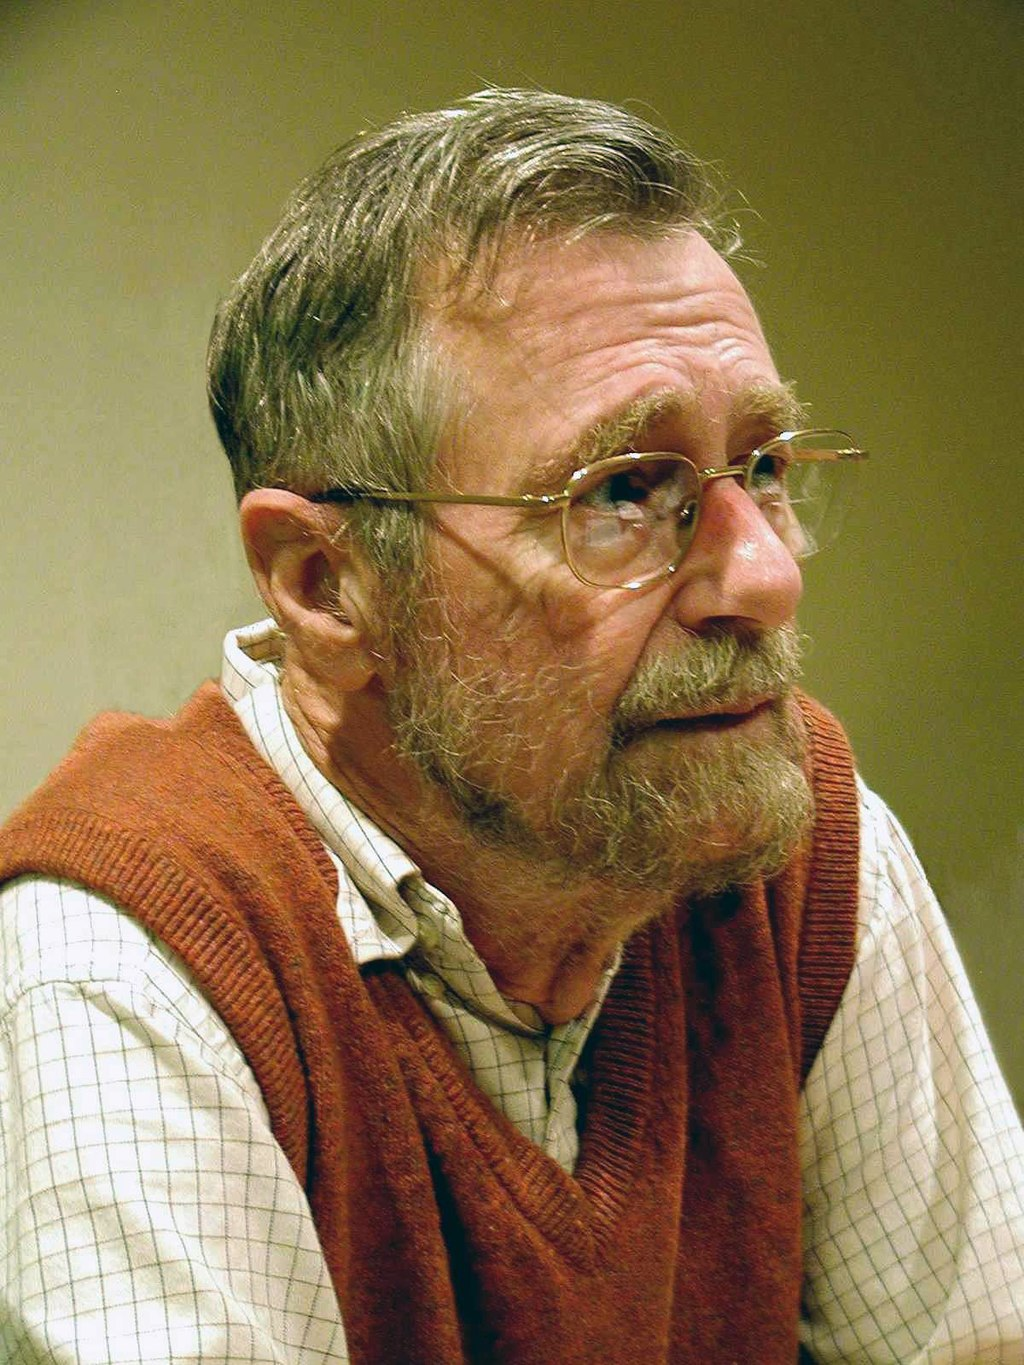
\includegraphics[width=0.35\textwidth]{Grundlagen_Info/02_Graphen/AbstraktionDurchGraphen/Figures/Edsger_Wybe_Dijkstra.jpg}
	\caption*{Edsger Wybe Dijkstra}
\end{figure}

\begin{figure}[H]
	\centering
	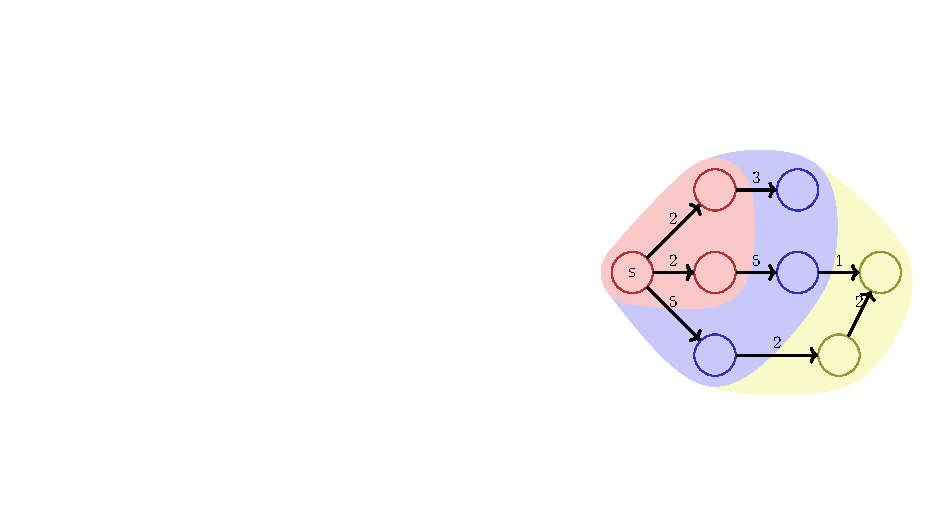
\includegraphics[width=0.6\textwidth]{Grundlagen_Info/02_Graphen/AbstraktionDurchGraphen/Figures/DScrop.pdf}
	\caption{Idee des Dijkstra-Algorithmus}
	\label{fig:wavefront}
\end{figure}

\noindent
Betrachten Sie zunächst einmal den Graphen in \cref{fig:wavefront}. Wir wählen einen beliebigen Knoten als Startknoten und nennen diesen $s$. Wir nehmen nun an, dass wir für einige Knoten bereits die Länge eines kürzesten Weges zu ihnen (von $s$ aus) bestimmt haben. Diese Knoten gehören zu der rot gefärbten Menge. Für die anderen Knoten (in den blau und gelb gefärbten Mengen), sind diese Längen noch nicht bekannt. Doch was unterscheidet die Knoten in der blauen von den Knoten in der gelben Menge? Die Knoten in der blauen Menge sind, im Gegensatz zu denen in der gelben, direkt (über eine einzige Kante) von mindestens einem der Knoten in der roten Menge erreichbar. Die Idee ist nun, dass wir die rote Menge systematisch um bestimmte Knoten aus der blauen Menge (\enquote{Wellenfront}) erweitern.

\noindent
Wir bezeichnen mit $d_s\lrs{v}$ die Länge des kürzesten \textbf{bisher} gefunden Weges vom Startknoten $s$ zum Knoten $v$. Mit $c(u,v)$ bezeichnen wir das Gewicht (cost) der Kante von Knoten $u$ zum Knoten $v$.
\begin{itemize}
	\item Zu Beginn: $d_s\lrs{v} = \infty$ für alle Knoten des Graphen. (Initialisierung)
	\item Ziel: Für jeden Knoten $v$ des Graphen soll am Ende $d_s\lrs{v}$ die Länge eines kürzesten Weges von $s$ nach $v$ sein.
\end{itemize}

\noindent
Wir beschreiben nun informal die Schritte des Dijkstra-Algorithmus.
\begin{itemize}
	\item Wir fügen $u:=s$ zur roten Menge hinzu und betrachten alle Knoten, welche direkt über eine einzige Kante von $s$ aus erreichbar sind (also genau die Knoten in der blauen Menge).
	\item Für jeden dieser blauen Knoten $v$ schauen wir, ob die Bedingung
	      \begin{align*}
		      d_s[u] + c(u,v) < d_s[v]
	      \end{align*}
	      erfüllt ist. Diese Bedingung hat die Bedeutung, dass die bislang berechneten Länge $d_s[v]$ grösser ist, als wenn wir von $s$ über $u$ nach $v$ gehen würden. Trifft diese zu, so führen wir das Update
	      \begin{align*}
		      d_s[v] = d_s[u] + c(u,v)
	      \end{align*}
	      durch und verbessern dadurch den bisherigen Wert $d_s[v]$.
	\item Nun wählen wir denjenigen blauen Knoten $u$, welchen den (einen der) kleinsten Werte $d_s[u]$ unter allen blauen Knoten hat, als den neuen Knoten $u$ und fügen $u$ zur roten Menge hinzu.
	\item Wir arbeiten nun so weiter, bis keine blauen Knoten mehr übrig sind.
\end{itemize}
Eine entscheidende Tatsache in dem Algorithmus (dies ist nicht völlig offensichtlich) ist, dass die roten Knoten $v$ ihren Wert $d_s[v]$ nie mehr ändern werden und dass für sie in der Tat  $d_s\lrs{v}$ die Länge eines kürzesten Weges von $s$ nach $v$ ist.


\begin{figure}[H]
	\centering
	\begin{subfigure}[b]{0.4\textwidth}
		\adjustbox{width=0.8\textwidth}{%
			\begin{tikzpicture}[
					node distance = 22mm and 24mm,
					every state/.append style = {inner sep=0pt, fill=gray!10,
							minimum size=11mm},
					every edge/.style = {draw, -Triangle, bend angle=15},
					auto=right,
				]
				\node (s) [state, fill=Yellow!50, align=center]         {$s$\\$0$};
				\node (t) [state, fill=Yellow!20, above right=of s,align=center]   {$t$\\$\infty$};
				\node (y) [state, fill=Yellow!20, below right=of s,align=center]         {$y$\\$\infty$};
				\node (x) [state, fill=Yellow!20, right=of t,align=center]   {$x$\\$\infty$};
				\node (z) [state, fill=Yellow!20, right=of y,align=center]   {$z$\\$\infty$};
				% %
				% \draw[gray!30, line width=5pt]
				%         (s1) to                     (s2)
				%         (s1) to [bend right=15]     (s6);
				% %
				\draw   (s) edge ["10"]             (t)
				(s) edge ["5"]              (y)
				(t) edge ["1"]              (x)
				(t) edge [bend right,"2"]    (y)
				(y) edge [bend right,"3"]   (t)
				(y) edge ["9"]  (x)
				(y) edge ["2"]             (z)
				(x) edge [bend right,"4"]  (z)
				(z) edge [very near end,"7"]  (s)
				(z) edge [bend right,"6"]    (x);
			\end{tikzpicture}
		}%
		\caption*{(a)}
	\end{subfigure}
	\begin{subfigure}[b]{0.4\textwidth}
		\adjustbox{width=0.8\textwidth}{%
			\begin{tikzpicture}[
					node distance = 22mm and 24mm,
					every state/.append style = {inner sep=0pt, fill=gray!10,
							minimum size=11mm},
					every edge/.style = {draw, -Triangle, bend angle=15},
					auto=right,
				]
				\node (s) [state,fill=Red!20, align=center]         {$s$\\$0$};
				\node (t) [state,fill=Blue!20, above right=of s,align=center]   {$t$\\$10$};
				\node (y) [state,fill=Blue!20, below right=of s,align=center]         {$y$\\$5$};
				\node (x) [state,fill=Yellow!20, right=of t,align=center]   {$x$\\$\infty$};
				\node (z) [state,fill=Yellow!20, right=of y,align=center]   {$z$\\$\infty$};
				% %
				% \draw[gray!30, line width=5pt]
				%         (s1) to                     (s2)
				%         (s1) to [bend right=15]     (s6);
				% %
				\draw   (s) edge ["10"]             (t)
				(s) edge ["5"]              (y)
				(t) edge ["1"]              (x)
				(t) edge [bend right,"2"]    (y)
				(y) edge [bend right,"3"]   (t)
				(y) edge ["9"]  (x)
				(y) edge ["2"]             (z)
				(x) edge [bend right,"4"]  (z)
				(z) edge [very near end,"7"]  (s)
				(z) edge [bend right,"6"]    (x);
			\end{tikzpicture}
		}%
		\caption*{(b)}
	\end{subfigure}


	\bigskip
	\begin{subfigure}[b]{0.4\textwidth}
		\adjustbox{width=0.8\textwidth}{%
			\begin{tikzpicture}[
					node distance = 22mm and 24mm,
					every state/.append style = {inner sep=0pt, fill=gray!10,
							minimum size=11mm},
					every edge/.style = {draw, -Triangle, bend angle=15},
					auto=right,
				]
				\node (s) [state, fill=Red!20, align=center]         {$s$\\$0$};
				\node (t) [state, fill=Blue!20, above right=of s,align=center]   {$t$\\$8$};
				\node (y) [state, fill=Red!20, below right=of s,align=center]         {$y$\\$5$};
				\node (x) [state, fill=Blue!20, right=of t,align=center]   {$x$\\$14$};
				\node (z) [state, fill=Blue!20, right=of y,align=center]   {$z$\\$7$};
				% %
				% \draw[gray!30, line width=5pt]
				%         (s1) to                     (s2)
				%         (s1) to [bend right=15]     (s6);
				% %
				\draw   (s) edge ["10"]             (t)
				(s) edge ["5"]              (y)
				(t) edge ["1"]              (x)
				(t) edge [bend right,"2"]    (y)
				(y) edge [bend right,"3"]   (t)
				(y) edge ["9"]  (x)
				(y) edge ["2"]             (z)
				(x) edge [bend right,"4"]  (z)
				(z) edge [very near end,"7"]  (s)
				(z) edge [bend right,"6"]    (x);
			\end{tikzpicture}
		}%
		\caption*{(c)}
	\end{subfigure}
	\begin{subfigure}[b]{0.4\textwidth}
		\adjustbox{width=0.8\textwidth}{%
			\begin{tikzpicture}[
					node distance = 22mm and 24mm,
					every state/.append style = {inner sep=0pt, fill=gray!10,
							minimum size=11mm},
					every edge/.style = {draw, -Triangle, bend angle=15},
					auto=right,
				]
				\node (s) [state, fill=Red!20, align=center]         {$s$\\$0$};
				\node (t) [state, fill=Blue!20, above right=of s,align=center]   {$t$\\$8$};
				\node (y) [state, fill=Red!20, below right=of s,align=center]         {$y$\\$5$};
				\node (x) [state, fill=Blue!20, right=of t,align=center]   {$x$\\$13$};
				\node (z) [state, fill=Red!20, right=of y,align=center]   {$z$\\$7$};
				% %
				% \draw[gray!30, line width=5pt]
				%         (s1) to                     (s2)
				%         (s1) to [bend right=15]     (s6);
				% %
				\draw   (s) edge ["10"]             (t)
				(s) edge ["5"]              (y)
				(t) edge ["1"]              (x)
				(t) edge [bend right,"2"]    (y)
				(y) edge [bend right,"3"]   (t)
				(y) edge ["9"]  (x)
				(y) edge ["2"]             (z)
				(x) edge [bend right,"4"]  (z)
				(z) edge [very near end,"7"]  (s)
				(z) edge [bend right,"6"]    (x);
			\end{tikzpicture}
		}%
		\caption*{(d)}
	\end{subfigure}

	\bigskip
	\begin{subfigure}[b]{0.4\textwidth}
		\adjustbox{width=0.8\textwidth}{%
			\begin{tikzpicture}[
					node distance = 22mm and 24mm,
					every state/.append style = {inner sep=0pt, fill=gray!10,
							minimum size=11mm},
					every edge/.style = {draw, -Triangle, bend angle=15},
					auto=right,
				]
				\node (s) [state, fill=Red!20, align=center]         {$s$\\$0$};
				\node (t) [state, fill=Red!20, above right=of s,align=center]   {$t$\\$8$};
				\node (y) [state, fill=Red!20, below right=of s,align=center]         {$y$\\$5$};
				\node (x) [state, fill=Blue!20, right=of t,align=center]   {$x$\\$9$};
				\node (z) [state, fill=Red!20, right=of y,align=center]   {$z$\\$7$};
				% %
				% \draw[gray!30, line width=5pt]
				%         (s1) to                     (s2)
				%         (s1) to [bend right=15]     (s6);
				% %
				\draw   (s) edge ["10"]             (t)
				(s) edge ["5"]              (y)
				(t) edge ["1"]              (x)
				(t) edge [bend right,"2"]    (y)
				(y) edge [bend right,"3"]   (t)
				(y) edge ["9"]  (x)
				(y) edge ["2"]             (z)
				(x) edge [bend right,"4"]  (z)
				(z) edge [very near end,"7"]  (s)
				(z) edge [bend right,"6"]    (x);
			\end{tikzpicture}
		}%
		\caption*{(e)}
	\end{subfigure}
	\begin{subfigure}[b]{0.4\textwidth}
		\adjustbox{width=0.8\textwidth}{%
			\begin{tikzpicture}[
					node distance = 22mm and 24mm,
					every state/.append style = {inner sep=0pt, fill=gray!10,
							minimum size=11mm},
					every edge/.style = {draw, -Triangle, bend angle=15},
					auto=right,
				]
				\node (s) [state, fill=Red!20, align=center]         {$s$\\$0$};
				\node (t) [state, fill=Red!20, above right=of s,align=center]   {$t$\\$8$};
				\node (y) [state, fill=Red!20, below right=of s,align=center]         {$y$\\$5$};
				\node (x) [state, fill=Red!20, right=of t,align=center]   {$x$\\$9$};
				\node (z) [state, fill=Red!20, right=of y,align=center]   {$z$\\$7$};
				% %
				% \draw[gray!30, line width=5pt]
				%         (s1) to                     (s2)
				%         (s1) to [bend right=15]     (s6);
				% %
				\draw   (s) edge ["10"]             (t)
				(s) edge ["5"]              (y)
				(t) edge ["1"]              (x)
				(t) edge [bend right,"2"]    (y)
				(y) edge [bend right,"3"]   (t)
				(y) edge ["9"]  (x)
				(y) edge ["2"]             (z)
				(x) edge [bend right,"4"]  (z)
				(z) edge [very near end,"7"]  (s)
				(z) edge [bend right,"6"]    (x);
			\end{tikzpicture}
		}%
		\caption*{(f)}
	\end{subfigure}
	\caption{vollständiges Beispiel für das Vorgehen des Dijkstra-Algorithmus mit $s$ als Startknoten}
	\label{fig:alg}
\end{figure}


\clearpage
\begin{myexercise}\label{aufgabe:205}
	Führen Sie die Schritte des Dijkstra-Algorithmus für den folgenden Graphen analog zu \cref{fig:alg} durch. Verwenden Sie $s$ als Startknoten der Berechnung.
	\begin{figure}[H]
		\centering
		\adjustbox{width=0.5\textwidth}{%
			\begin{tikzpicture}[
					node distance = 22mm and 24mm,
					every state/.append style = {inner sep=0pt, fill=gray!10,
							minimum size=11mm},
					every edge/.style = {draw, -Triangle, bend angle=15},
					auto=right,
				]
				\node (s) [state, align=center]         {$s$};
				\node (t) [state, above right=of s,align=center]   {$t$};
				\node (y) [state, below right=of s,align=center]         {$y$};
				\node (x) [state, right=of t,align=center]   {$x$};
				\node (z) [state, right=of y,align=center]   {$z$};
				% %
				% \draw[gray!30, line width=5pt]
				%         (s1) to                     (s2)
				%         (s1) to [bend right=15]     (s6);
				% %
				\draw   (s) edge ["3"]             (t)
				(s) edge ["5"]              (y)
				(t) edge ["6"]              (x)
				(t) edge [bend right,"2"]    (y)
				(y) edge [bend right,"1"]   (t)
				(y) edge ["4"]  (x)
				(y) edge ["6"]             (z)
				(x) edge [bend right,"2"]  (z)
				(z) edge [very near end,"3"]  (s)
				(z) edge [bend right,"7"]    (x);
			\end{tikzpicture}
		}%
	\end{figure}
	\begin{myanswer}\label{aufgabe:205-sol}
		\begin{figure}[H]
			\centering
			\begin{subfigure}[b]{0.4\textwidth}
				\adjustbox{width=0.8\textwidth}{%
					\begin{tikzpicture}[
							node distance = 22mm and 24mm,
							every state/.append style = {inner sep=0pt, fill=gray!10,
									minimum size=11mm},
							every edge/.style = {draw, -Triangle, bend angle=15},
							auto=right,
						]
						\node (s) [state, fill=Yellow!50, align=center]         {$s$\\$0$};
						\node (t) [state, fill=Yellow!20, above right=of s,align=center]   {$t$\\$\infty$};
						\node (y) [state, fill=Yellow!20, below right=of s,align=center]         {$y$\\$\infty$};
						\node (x) [state, fill=Yellow!20, right=of t,align=center]   {$x$\\$\infty$};
						\node (z) [state, fill=Yellow!20, right=of y,align=center]   {$z$\\$\infty$};
						% %
						% \draw[gray!30, line width=5pt]
						%         (s1) to                     (s2)
						%         (s1) to [bend right=15]     (s6);
						% %
						\draw   (s) edge ["3"]             (t)
						(s) edge ["5"]              (y)
						(t) edge ["6"]              (x)
						(t) edge [bend right,"2"]    (y)
						(y) edge [bend right,"1"]   (t)
						(y) edge ["4"]  (x)
						(y) edge ["6"]             (z)
						(x) edge [bend right,"2"]  (z)
						(z) edge [very near end,"3"]  (s)
						(z) edge [bend right,"7"]    (x);
					\end{tikzpicture}
				}%
				\caption*{(a)}
			\end{subfigure}
			\begin{subfigure}[b]{0.4\textwidth}
				\adjustbox{width=0.8\textwidth}{%
					\begin{tikzpicture}[
							node distance = 22mm and 24mm,
							every state/.append style = {inner sep=0pt, fill=gray!10,
									minimum size=11mm},
							every edge/.style = {draw, -Triangle, bend angle=15},
							auto=right,
						]
						\node (s) [state,fill=Red!20, align=center]         {$s$\\$0$};
						\node (t) [state,fill=Blue!20, above right=of s,align=center]   {$t$\\$3$};
						\node (y) [state,fill=Blue!20, below right=of s,align=center]         {$y$\\$5$};
						\node (x) [state,fill=Yellow!20, right=of t,align=center]   {$x$\\$\infty$};
						\node (z) [state,fill=Yellow!20, right=of y,align=center]   {$z$\\$\infty$};
						% %
						% \draw[gray!30, line width=5pt]
						%         (s1) to                     (s2)
						%         (s1) to [bend right=15]     (s6);
						% %
						\draw   (s) edge ["3"]             (t)
						(s) edge ["5"]              (y)
						(t) edge ["6"]              (x)
						(t) edge [bend right,"2"]    (y)
						(y) edge [bend right,"1"]   (t)
						(y) edge ["4"]  (x)
						(y) edge ["6"]             (z)
						(x) edge [bend right,"2"]  (z)
						(z) edge [very near end,"3"]  (s)
						(z) edge [bend right,"7"]    (x);
					\end{tikzpicture}
				}%
				\caption*{(b)}
			\end{subfigure}


			\bigskip
			\begin{subfigure}[b]{0.4\textwidth}
				\adjustbox{width=0.8\textwidth}{%
					\begin{tikzpicture}[
							node distance = 22mm and 24mm,
							every state/.append style = {inner sep=0pt, fill=gray!10,
									minimum size=11mm},
							every edge/.style = {draw, -Triangle, bend angle=15},
							auto=right,
						]
						\node (s) [state,fill=Red!20, align=center]         {$s$\\$0$};
						\node (t) [state,fill=Red!20, above right=of s,align=center]   {$t$\\$3$};
						\node (y) [state,fill=Blue!20, below right=of s,align=center]         {$y$\\$5$};
						\node (x) [state,fill=Blue!20, right=of t,align=center]   {$x$\\$9$};
						\node (z) [state,fill=Yellow!20, right=of y,align=center]   {$z$\\$\infty$};
						% %
						% \draw[gray!30, line width=5pt]
						%         (s1) to                     (s2)
						%         (s1) to [bend right=15]     (s6);
						% %
						\draw   (s) edge ["3"]             (t)
						(s) edge ["5"]              (y)
						(t) edge ["6"]              (x)
						(t) edge [bend right,"2"]    (y)
						(y) edge [bend right,"1"]   (t)
						(y) edge ["4"]  (x)
						(y) edge ["6"]             (z)
						(x) edge [bend right,"2"]  (z)
						(z) edge [very near end,"3"]  (s)
						(z) edge [bend right,"7"]    (x);
					\end{tikzpicture}
				}%
				\caption*{(c)}
			\end{subfigure}
			\begin{subfigure}[b]{0.4\textwidth}
				\adjustbox{width=0.8\textwidth}{%
					\begin{tikzpicture}[
							node distance = 22mm and 24mm,
							every state/.append style = {inner sep=0pt, fill=gray!10,
									minimum size=11mm},
							every edge/.style = {draw, -Triangle, bend angle=15},
							auto=right,
						]
						\node (s) [state,fill=Red!20, align=center]         {$s$\\$0$};
						\node (t) [state,fill=Red!20, above right=of s,align=center]   {$t$\\$3$};
						\node (y) [state,fill=Red!20, below right=of s,align=center]         {$y$\\$5$};
						\node (x) [state,fill=Blue!20, right=of t,align=center]   {$x$\\$9$};
						\node (z) [state,fill=Blue!20, right=of y,align=center]   {$z$\\$11$};
						% %
						% \draw[gray!30, line width=5pt]
						%         (s1) to                     (s2)
						%         (s1) to [bend right=15]     (s6);
						% %
						\draw   (s) edge ["3"]             (t)
						(s) edge ["5"]              (y)
						(t) edge ["6"]              (x)
						(t) edge [bend right,"2"]    (y)
						(y) edge [bend right,"1"]   (t)
						(y) edge ["4"]  (x)
						(y) edge ["6"]             (z)
						(x) edge [bend right,"2"]  (z)
						(z) edge [very near end,"3"]  (s)
						(z) edge [bend right,"7"]    (x);
					\end{tikzpicture}
				}%
				\caption*{(d)}
			\end{subfigure}

			\bigskip
			\begin{subfigure}[b]{0.4\textwidth}
				\adjustbox{width=0.8\textwidth}{%
					\begin{tikzpicture}[
							node distance = 22mm and 24mm,
							every state/.append style = {inner sep=0pt, fill=gray!10,
									minimum size=11mm},
							every edge/.style = {draw, -Triangle, bend angle=15},
							auto=right,
						]
						\node (s) [state,fill=Red!20, align=center]         {$s$\\$0$};
						\node (t) [state,fill=Red!20, above right=of s,align=center]   {$t$\\$3$};
						\node (y) [state,fill=Red!20, below right=of s,align=center]         {$y$\\$5$};
						\node (x) [state,fill=Red!20, right=of t,align=center]   {$x$\\$9$};
						\node (z) [state,fill=Blue!20, right=of y,align=center]   {$z$\\$11$};
						% %
						% \draw[gray!30, line width=5pt]
						%         (s1) to                     (s2)
						%         (s1) to [bend right=15]     (s6);
						% %
						\draw   (s) edge ["3"]             (t)
						(s) edge ["5"]              (y)
						(t) edge ["6"]              (x)
						(t) edge [bend right,"2"]    (y)
						(y) edge [bend right,"1"]   (t)
						(y) edge ["4"]  (x)
						(y) edge ["6"]             (z)
						(x) edge [bend right,"2"]  (z)
						(z) edge [very near end,"3"]  (s)
						(z) edge [bend right,"7"]    (x);
					\end{tikzpicture}
				}%
				\caption*{(e)}
			\end{subfigure}
			\begin{subfigure}[b]{0.4\textwidth}
				\adjustbox{width=0.8\textwidth}{%
					\begin{tikzpicture}[
							node distance = 22mm and 24mm,
							every state/.append style = {inner sep=0pt, fill=gray!10,
									minimum size=11mm},
							every edge/.style = {draw, -Triangle, bend angle=15},
							auto=right,
						]
						\node (s) [state,fill=Red!20, align=center]         {$s$\\$0$};
						\node (t) [state,fill=Red!20, above right=of s,align=center]   {$t$\\$3$};
						\node (y) [state,fill=Red!20, below right=of s,align=center]         {$y$\\$5$};
						\node (x) [state,fill=Red!20, right=of t,align=center]   {$x$\\$9$};
						\node (z) [state,fill=Red!20, right=of y,align=center]   {$z$\\$11$};
						% %
						% \draw[gray!30, line width=5pt]
						%         (s1) to                     (s2)
						%         (s1) to [bend right=15]     (s6);
						% %
						\draw   (s) edge ["3"]             (t)
						(s) edge ["5"]              (y)
						(t) edge ["6"]              (x)
						(t) edge [bend right,"2"]    (y)
						(y) edge [bend right,"1"]   (t)
						(y) edge ["4"]  (x)
						(y) edge ["6"]             (z)
						(x) edge [bend right,"2"]  (z)
						(z) edge [very near end,"3"]  (s)
						(z) edge [bend right,"7"]    (x);
					\end{tikzpicture}
				}%
				\caption*{(f)}
			\end{subfigure}
		\end{figure}
	\end{myanswer}
\end{myexercise}


\begin{myexercise}\label{aufgabe:206}
	Bislang konnten wir mit dem Dijkstra-Algorithmus lediglich die Längen der kürzesten Wege berechnen. Natürlich möchten wir aber auch die eigentlichen kürzesten Wege (die Folge von Knoten und Kanten) in Erfahrung bringen. Was müssen Sie an dem bisherigen Vorgehen ändern, damit nach Durchführung des Algorithmus die eigentlichen Wege zurückverfolgt werden können?
	\begin{myanswer}\label{aufgabe:206-sol}
		Die Idee der Strategie lässt sich recht einfach beschreiben. Betrachten wir einen beliebigen Knoten $v$ im Graphen, der nicht der Startknote ist. Zu Beginn ist der bisherige Wert für den kürzesten Weg nach $v$ auf $\infty$ gesetzt. Falls $v$ von $s$ aus überhaupt erreichbar ist, dann wird dieser Wert im Verlaufe des Algorithmus irgendwann auf einen endlichen Wert gesetzt. Damit dies passieren kann, muss es einen Knoten geben (möglicherweise $s$), über den es eine günstigere Verbindung von $s$ nach $v$ gibt. Denn genau dann wird dieser ursprünglich unendliche Wert im Update-Schritt angepasst.

		Jedes Mal wenn der Wert von $v$ ein Update bekommt, speichern wir ab, von welchem Vorgängerknoten dieses Update erfolgte. Erfolgen mehrere Updates, so überschreiben wir diesen Vorgängerknoten jedes Mal. Am Ende haben wir uns für jeden Knoten $v$ gemerkt, über welchen Knoten $u$ er auf einem kürzesten Weg erreicht wurde. Doch die analogen Informationen haben wir uns auch für $u$ gemerkt und so weiter. Auf diese Weise können wir der Kette der Vorgängerknoten folgen und einen kürzesten Weg von $s$ nach $v$ rekonstruieren.
	\end{myanswer}
\end{myexercise}

\section{Weitere Aufgaben}
\begin{myexercise}\label{aufgabe:290}
	Wir nehmen an, dass ein Graph nur positive Kantengewichte besitzt. Kann in diesem Graphen ein kürzester Weg von Knoten $s$ nach Knoten $t$ eine Schleife (einen \textit{Zyklus}) enthalten?
	\begin{figure}[H]
		\centering
		\begin{tikzpicture}[
				node distance = 10mm and 12mm,
				every state/.append style = {inner sep=0pt, fill=gray!10,
						minimum size=8mm},
				every edge/.style = {draw, -Triangle, bend angle=15},
				auto=right,
			]
			\node (s) [state,fill=Blue!20,align=center]         {$s$};
			\node (u) [state, right=of s,align=center]   {$u$};
			\node (v) [state, above right=of u,align=center]         {$v$};
			\node (t) [state,fill=Green!20,below right=of v,align=center]   {$t$};
			\node (w) [state, below right=of u,align=center]   {$w$};
			% %
			% \draw[gray!30, line width=5pt]
			%         (s1) to                     (s2)
			%         (s1) to [bend right=15]     (s6);
			% %
			\draw   (s) edge ["1",color=Blue] (u)
			(u) edge ["1",color=Blue] (v)
			(v) edge ["1",color=Blue] (t)
			(v) edge ["1"] (w)
			(w) edge ["2"] (u)
			(w) edge ["4"] (t);
		\end{tikzpicture}
	\end{figure}
	\noindent
	Zum Beispiel ist $\textcolor{Red}{ v \longrightarrow w \longrightarrow u \longrightarrow v}$ ein Zyklus in diesem Graphen. Begründen Sie Ihre Antwort präzise.
	\begin{myanswer}\label{aufgabe:290-sol}
		\begin{figure}[H]
			\centering
			\begin{tikzpicture}[
					node distance = 10mm and 12mm,
					every state/.append style = {inner sep=0pt, fill=gray!10,
							minimum size=8mm},
					every edge/.style = {draw, -Triangle, bend angle=15},
					auto=right,
				]
				\node (s) [state,fill=Blue!20,align=center]         {$s$};
				\node (u) [state, right=of s,align=center]   {$u$};
				\node (v) [state, above right=of u,align=center]         {$v$};
				\node (t) [state,fill=Green!20,below right=of v,align=center]   {$t$};
				\node (w) [state, below right=of u,align=center]   {$w$};
				% %
				% \draw[gray!30, line width=5pt]
				%         (s1) to                     (s2)
				%         (s1) to [bend right=15]     (s6);
				% %
				\draw   (s) edge ["1",color=Blue] (u)
				(u) edge ["1",color=Blue] (v)
				(v) edge ["1",color=Blue] (t)
				(v) edge ["1"] (w)
				(w) edge ["2"] (u)
				(w) edge ["4"] (t);
			\end{tikzpicture}
		\end{figure}
		\begin{align*}
			 & \textcolor{Blue}{s \longrightarrow u \longrightarrow v \longrightarrow t}                                                                                            \\
			 & \textcolor{Blue}{s \longrightarrow u \longrightarrow} \textcolor{Red}{ v \longrightarrow w \longrightarrow u \longrightarrow v} \textcolor{Blue}{\longrightarrow  t} \\
		\end{align*}
		Ein Zyklus (hier: $\textcolor{Red}{ v \longrightarrow w \longrightarrow u \longrightarrow v}$) macht den Weg unnötig lange! Wir können den Zyklus einfach weglassen. Kürzeste Wege enthalten keine Zyklen.
	\end{myanswer}
\end{myexercise}

% \begin{myexercise}\label{aufgabe:291}
% (Challenge) Skizzieren Sie einen Graphen, genauer gesagt eine Folge von Graphen, sodass die Anzahl der Wege (ohne Zyk
% Im Unterricht haben wir erwähnt, dass mit wachsender 

% es unrealistisch (praktisch nicht durchführbar) ist
% \end{myexercise}

\clearpage

\section{Der Dijkstra-Algorithmus in Pseudocode}
Wir bezeichnen mit $d_s\lrs{v}$ die Länge des kürzesten \textbf{bisher} gefunden Weges vom Startknoten $s$ zum Knoten $v$.
\begin{itemize}
	\item Zu Beginn: $d_s\lrs{v} = \infty$ für alle Knoten des Graphen.
	\item Ziel: Für jeden Knoten $v$ des Graphen soll am Ende $d_s\lrs{v}$ die Länge eines kürzesten Weges von $s$ nach $v$ sein.
\end{itemize}
\begin{lstlisting}[language=Python,numbers=none,escapeinside={(*}{*)}]
### Dijkstra-Algorithmus ###

## Initialisierung ##
für alle Knoten u des Graphen setze:
    (*$d_s[u] = \infty$*)
(*$d_s[s] \leftarrow 0$*)
(*$S \leftarrow \emptyset$*)
(*$Q \leftarrow $*) Menge aller Knoten des Graphen

## Schritte ##
solange (*$Q$*) nicht leer ist, mach:
    (*$u\leftarrow$*) Knoten aus (*$Q$*) mit kleinstem (*$d_s[u]$*)
    (*$Q \leftarrow Q \setminus \lrc{u}$*)
    (*$S\leftarrow S \cup \lrc{u}$*)

    für alle von (*$u$*) direkt erreichbaren Knoten (*$v$*) mach:
        # ist der Weg von (*$s$*) nach (*$v$*) kürzer über (*$u$*)?
        falls (*$d_s[u] + c(u,v) < d_s[v]$*) dann:
            (*$d_s[v] \leftarrow d_s[u] + c(u,v)$*)
\end{lstlisting}

\shipoutAnswer